\subsection{Qualititave Measures of Prediction Quality}
\label{subsec:results_quality}

For side chain prediction experiments, 85.2\% of side chain prediction conformations (9406 of 11030 total) predicted with the new cell based solvation model are within 0.2 angstrom heavy atom RMSD of the prediction using the naive implementation.
In other metrics, the quality of prediction is comparable between the two solvent models. 
Median side chain heavy atom RMSD is 0.567 and 0.558 angstroms for the cell based method and the non-cell based method, respectively.
Average RMSD to the crystal structure is similarly close, 1.11 angstroms for both methods, with 79.9\% of side chain predictions within 2 angstroms RMSD of the native using the cell based model and 79.4\% within two angstroms using the naive approach.
Of side chains that are predicted differently by the two implementations there is no correlation between solvation model and prediction quality.
The distribution of side chain predictions with respect to RMSD to native is also indistinguishable between the two methods of computing the solvation term.

Data for energy calculations is not presented here because it is identical in every case.
This is expected, given that the two models represent two methods of computing the same quantity.
Thus, on the whole, prediction accuracy of the hash based model is comparable with the old implementation.

\subsection{Performance Improvement}
\label{subsec:performance_improvement}

% side by side performance comparison figure
\begin{figure}[h]
\centering
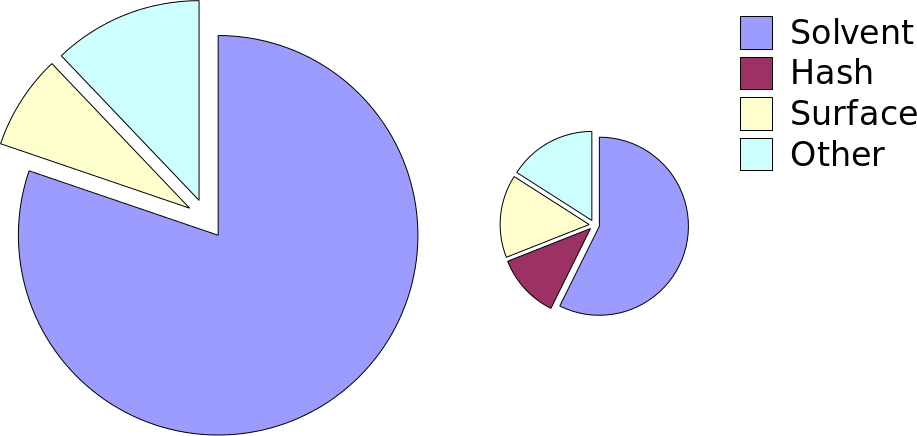
\includegraphics[width=0.6\textwidth]{figures/side_by_side.png}
\caption{Time spent during energy calculations on different parts of the energy model.
The left pie represents the non-cell based approach and the right pie the cell based approach.
The charts are scaled relative to the total cost of computing the energy.
Although some overhead is introduced in maintaining the hash structure, magenta, this significantly reduces the total cost of the solvent term, and as the solvent is such a large contributor to the total, the total cost of computing the energy is also significantly reduced.}
\label{figure:timing_pie}
\end{figure}

The principal goal of the hash based approach is to improve the performance of the implicit solvent models. 
Thus, the key metric of performance improvement is the speedup over the previous implementation.
Energy computations were found to be from 1.6 to 2.5 times as fast, and the trend indicates that even larger improvements would be obtained on calculations on larger system, see figure \ref{figure:grid_based_performance}.
A direct energy calculation experiment, as performed here, represents a ``best case'' for the expected performance increase of a hash based solvent, as these experiments minimize the fraction of time spent in other types of calculations.
Implicit solvent calculations, and energy calculations in general, compose a smaller fraction of time in simultaneous side chain prediction.
Therefore, the observed performance improvement is less than that of energy calculations.
The observed performance increase in this sort of experiment is still on the order of 20\%.
Figure \ref{figure:timing_pie}, illustrates the fraction of time spent during an energy calculation on different terms of the energy model, as well as the improvement, and change in proportions using a grid based model.
                                                                      
\begin{figure}[H]
\centering
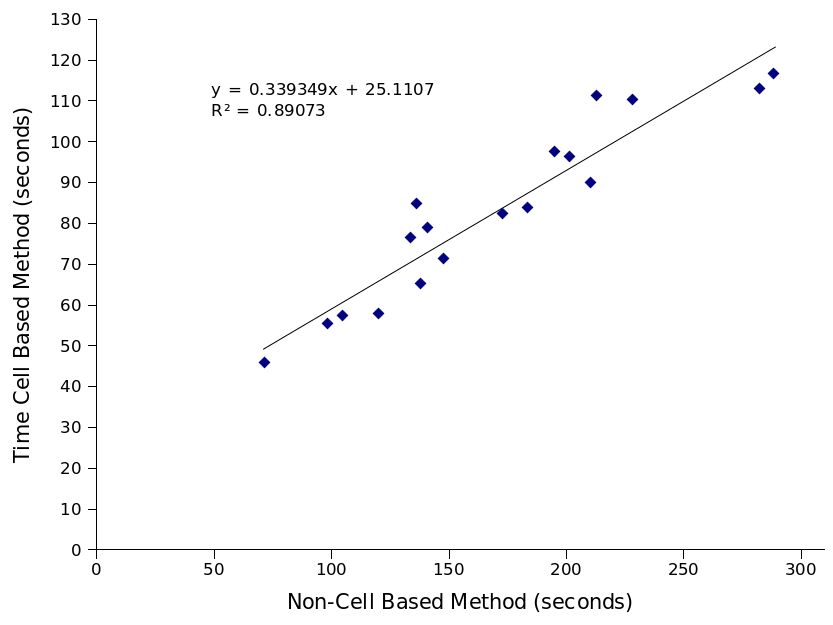
\includegraphics[width=0.8\textwidth]{figures/energy_calculation_timings.png}
\caption{The general trend in energy calculation time as a function of system size, each point represents a single system.
Energy computations using a grid based method yield approximately a three times performance improvement, slope of 0.339.
However, in the case of some very small structures, it is possible that the overhead introduced by maintaining the grid structure outweighs the improvement.
Performance for small systems is already very good, and thus the improvement in larger systems is far more valuable than the small penalty paid in small systems.}
\label{figure:grid_based_performance}
\end{figure}

\begin{table}[H]
\centering
\label{table:energy_timings}
\begin{tabular}{|c|c|c|}
\hline
PDB id	& Naive Method	& Cell Based Method	\\
\hline
1F5Z	&  201.75	&  96.37	\\
1H2V	&  98.31	&  55.32	\\
1HRD	&  228.38	&  110.12	\\
1M1Z	&  147.83	&  71.28	\\
1M9X	&  282.35	&  113.04	\\
1O60	&  172.82	&  82.34	\\
1R0V	&  210.35	&  90.0  \\
1XMP	&  213.25	&  111.25	\\
2E3Z	&  141.11	&  78.79	\\
2H6U	&  138.25	&  65.07	\\
2OU1	&  104.93	&  57.24	\\
2XI9	&  71.68	&  45.73	\\
3AMD	&  288.58	&  116.52	\\
3DEL	&  133.62	&  76.48	\\
3E1E	&  183.8	&  83.8	\\
3FGN	&  120.38	&  57.75	\\
3HHP	&  195.25	&  97.58	\\
4GVR	&  136.35	&  84.78	\\
\hline
\end{tabular}
\caption{The specific experimental times for a series of energy computations presented in Figure \ref{figure:grid_based_performance}.
These examples represent a ``best case'' scenario, as the majority of time in these experiments is spent computing the solvent contribution, and thus the improvement is more evident.}
\end{table}
% Would it be useful in this table to add a column that shows %improvement?



